%!TEX root = ../thesis.tex
\chapter{Background}
\label{chap:background}
\nocite{*}


\section{Pairs Trading}

Pairs trading is a market-neutral trading strategy that matches a long position with a short position in a pair of highly correlated instruments such as two stocks, exchange-traded funds (ETFs), currencies, commodities or options. Pairs traders wait for weakness in the correlation and then go long the under-performer while simultaneously short selling the over-performer, closing the positions as the relationship returns to statistical norms.\cite{investo:pairs}


\subsection{Cointegration Test}

In order to find pairs to trade in pairs trading, we look for cointegrated relationship in pairs. A pair is cointegrated if individual instruments are of same order and the linear combination of them is stationary. We test stationarity of the linear combination of the pair, say \(y_t\). Stationarity is referred as weak stationarity in this case that a series is stationary if the mean and autocovariance are independent of time and the variance is finite for all times.\cite{wiki:stationarity} We simply regress \(y_t\) on its lagged values \(y_{t-1}\) and find out whether the coefficient \(\phi\) is 1 or not. Consider autoregressive process of order 1, AR(1), as shown:\cite{study:coint}
\begin{equation}
y_t = \phi y_{t-1} + \epsilon_t
\end{equation}
where \(\epsilon_t\) is white noise error term with mean zero and constant variance. Then,
\begin{equation}
\Delta y_t = \delta y_{t-1} + \epsilon_t
\end{equation}
where \(\Delta\) is first difference and \(\delta = \phi - 1\). If \(\delta = 0\), then \(\Delta y_t = \epsilon_t \), it means \(y_t\) is random walk and non-stationary. Otherwise, it is a stationary process. This is called Dickey-Fuller Test.

Moreoever, we have Augmented Dickey-Fuller (ADF) Test, which allows for higher-order autoregressive processes, as shown:\cite{study:coint}
\begin{equation}
\Delta y_t = \alpha + \beta t + \gamma y_{t-1} + \sum_{j=1}^{p} \delta_j \Delta y_{t-j} + \epsilon_t
\end{equation}

For this model, we test for the null hypothesis as \(H_0: \gamma = 0\) against alternative hypothesis as \(H_1: \gamma < 0\). We reject the null if the test statistic is smaller than critical value of a significance level. 

In this project, we use ADF test to check cointegration of two stock price series. We construct linear combination of two stock price series as:
\begin{equation}
y_t = S_t^1 - a S_t^2
\end{equation}
where \(S_t^1\) and \(S_t^2\) are price series of stock 1 and stock 2.


\subsection{Bollinger Band Strategy}

Bollinger band strategy is typically used in pairs trading to capture profit between upper and lower bands. Upper and lower band are constructed 1-2 standard deviations from the moving average of the series \(y_t\).\cite{pairstrading} There are also many ways of entry and exit, long and short. In our trading model, we long when \(y_t\) crosses down the lower band, short when \(y_t\) crosses up the upper band, where the profit is captured between buy and sell points, as shown in Figure 2.1.

\begin{figure}[h!]
\centering
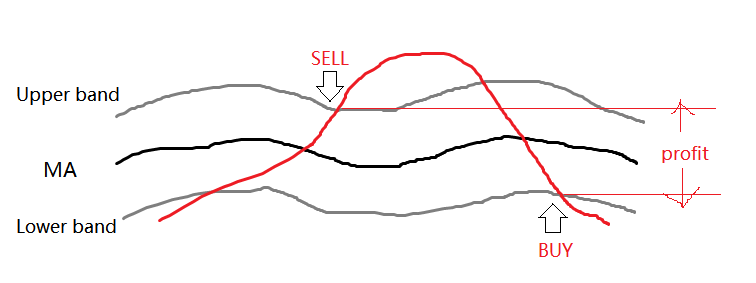
\includegraphics{background/images/bollinger.png}
\caption{Bollinger Band}
\label{fig:bollinger}
\end{figure}



\section{Machine Learning}

\subsection{Principle Component Analysis}

Principle Component Analysis (PCA) is used for reducing the number of variables comprising a dataset while retaining the variability in the data, or identifying hidden patterns in the data, and classifying them according to how much of the information, stored in the data, they account for.\cite{pca} We use PCA for our stock market data for both purposes. 

We take stock price panel data as score matrix \(A\), and coefficient vector \(l\) that generates linear combination on \(A\) which yields principle components \(Y\) of smaller dimension than \(A\). Principle components \(Y\) are independent and each coefficient vector \(l_i\) is required to maximize the variance of its corresponding principle component \(Y_i\), as shown:\cite{pca}
\begin{equation}
\max{Var(Y_i) = l_i^T C l_i}
\end{equation}
\[s.t.\]
\[||l_i^T|| = 1, \forall i\]
\[l_i^T l_j = 0, \forall j\neq i\]
which has Lagrangian form:
\begin{equation}
L(l_i, \lambda_i, \delta) = l_i^T C l_i - \lambda_i(l_i^T l_i - 1) - \delta(l_i^T l_i)
\end{equation}
Maximizing L by taking partial derivatives to 0, we obtain \(C l_i = \lambda_i l_i\), where \(C\) is covariance matrix of \(A\) and \(\lambda_i, l_i\) are corresponding eigenvalues and eigenvectors. 

Therefore, principle components are constructed from eigenvectors of score matrix with score matrix itself: \(Y_i = l_i^T A\).


\subsection{DBSCAN Clustering}

\begin{figure}[h!]
\centering
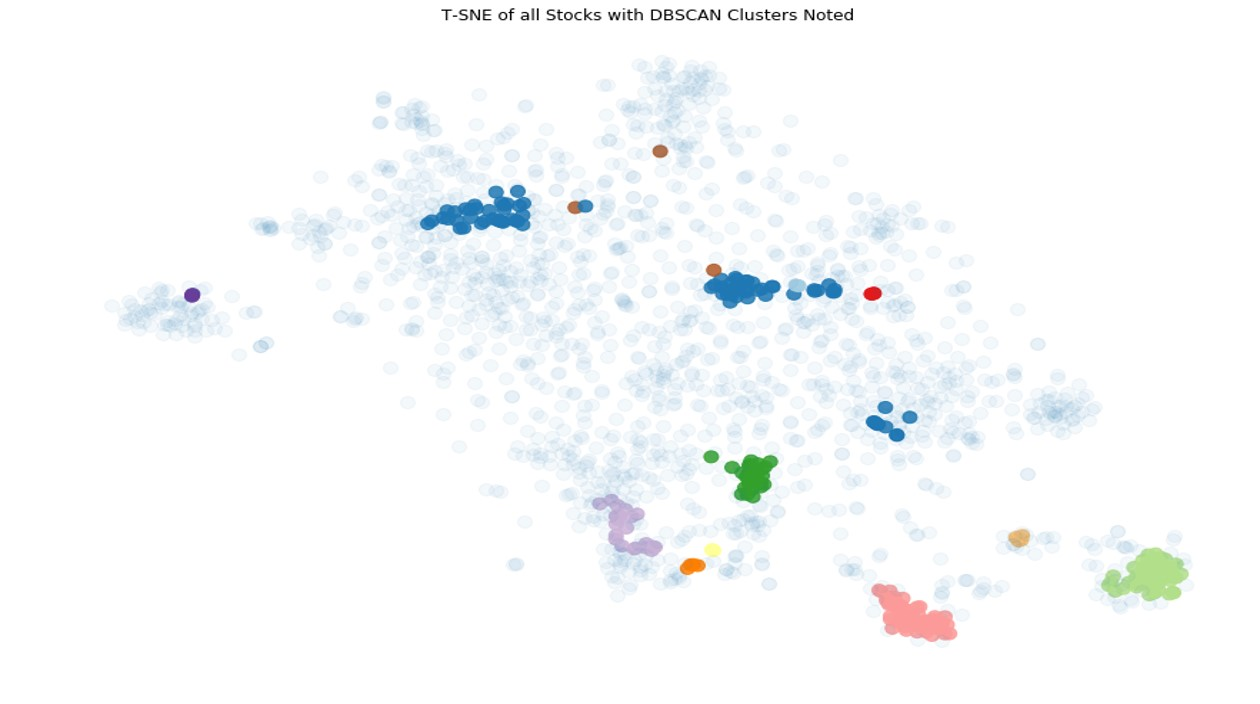
\includegraphics[scale=0.4]{background/images/Clustering.jpg}
\caption{DBSCAN Clustering}
\label{fig:cluster}
\end{figure}

Density-based spatial clustering of applications with noise (DBSCAN) is a density-based clustering non-parametric algorithm: given a set of points in some space, it groups together points that are closely packed together (points with many nearby neighbors).\cite{wiki:dbscan} Unlike normal clustering method that group all points, DBSCAN does not group outliers that lie alone in low-density regions. Another characteristic of DBSCAN is that it is likely to produce different clusters at each run. An example is shown in Figure 2.1.

DBSCAN has two important hyperparameters. Minimum sample size is minimum number of points in a group. Distance parameter is largest distance between points in a group. We pick \( \epsilon = 1.8, min samples = 3\) to get a reasonable number of resulting clusters, which is about 8 clusters.
